%%%%%%%%%%%%%%%%%%%%%%% file template.tex %%%%%%%%%%%%%%%%%%%%%%%%%
%
% This is a general template file for the LaTeX package SVJour3
% for Springer journals.          Springer Heidelberg 2006/03/15
%
% Copy it to a new file with a new name and use it as the basis
% for your article. Delete % signs as needed.
%
% This template includes a few options for different layouts and
% content for various journals. Please consult a previous issue of
% your journal as needed.
%
%%%%%%%%%%%%%%%%%%%%%%%%%%%%%%%%%%%%%%%%%%%%%%%%%%%%%%%%%%%%%%%%%%%
%
% First comes an example EPS file -- just ignore it and
% proceed on the \documentclass line
% your LaTeX will extract the file if required
%
%\documentclass{svjour3}                     % onecolumn (standard format)
%\documentclass[smallextended]{svjour3}     % onecolumn (second format)
\documentclass[twocolumn]{svjour3}         % twocolumn
%
\smartqed  % flush right qed marks, e.g. at end of proof
%
\usepackage{graphicx}
%
% \usepackage{mathptmx}      % use Times fonts if available on your TeX system
%
% insert here the call for the packages your document requires
%\usepackage{latexsym}
% etc.
%
% please place your own definitions here and don't use \def but
% \newcommand{}{}
%
% Insert the name of "your journal" with
% \journalname{myjournal}
%
\begin{document}

\title{Towards cross-middleware authentication and single sign-on for ARC Grid middleware
%\thanks{Grants or other notes
%about the article that should go on the front page should be
%placed here. General acknowledgments should be placed at the end of the article.}
}
\subtitle{Do you have a subtitle?\\ If so, write it here}

%\titlerunning{Short form of title}        % if too long for running head

\author{Weizhong Qiang         \and
        Aleksandr Konstantinov %etc.
}

%\authorrunning{Short form of author list} % if too long for running head

\institute{F. Author \at
              first address \\
              Tel.: +123-45-678910\\
              Fax: +123-45-678910\\
              \email{fauthor@example.com}           %  \\
%             \emph{Present address:} of F. Author  %  if needed
           \and
           S. Author \at
              second address
}

\date{Received: date / Accepted: date}
% The correct dates will be entered by the editor


\maketitle

\begin{abstract}
When pursuing the task of making access to Grids as simple as possible, security is one of the most important challenges in production Grid infrastructures, especially when the Grid applications span multiple administrative domains as well as heterogeneous Grid middlewares. A typical example is wide scale e-Science applications which need to coordinate resources shared among a number of independent institutions with different Grid middlewares deployed on these resources. In this paper, we describe security implementation and considerations used in the upcoming version of the Advanced Resource Connector (ARC) middleware, where the heterogeneity issue has been addressed. The main goal of ARC implementation in terms of security is to let the middleware be capable of interoperating with other Grid middlewares by leveraging on standard specifications. The key aspect of the work is to enhance the current proxy certificate based authentication and single sign-on by utilizing and enhancing the standardized Web Service specifications such as Security Assertion Markup Languages (SAML), single sign-on (SSO) profile and Web Services Security in order to achieve cross-middleware authentication and single sign-on.
\keywords{single sign-on \and delegation \and virtual organization \and ARC middleware }
% \PACS{PACS code1 \and PACS code2 \and more}
% \subclass{MSC code1 \and MSC code2 \and more}
\end{abstract}

\section{Introduction} 
\label{sec:intro}
Grid provides the technology for wide-scale, cross-domain collaboration where users work with resources and share data which are distributed across administrative domains. This kind of collaboration is called Virtual Organization (VO)~\cite{IFoster01}. The resources that contribute to the VO can come from independent administrative domains, and even require different security approaches to access control due to usage of different underlying middlewares. The same heterogeneous situation applies to users who need to access the VO resources, because users holding one kind of a credential may need to utilize multiple resources with different security approaches. To solve the above issues, Grid middlewares should provide the following abilities:
The user which participates a VO should be able to access data and resources without being required to constantly do authentication at each resource or service;
The VO should be able to easily manage the privileges and memberships of the users;
The VO together with its resources should be able to easily manage the authorization, given the condition that the resources are owned by different administrative domains.

In the current Grid community, the Grid Security Infrastructure (GSI)~\cite{IFoster98} is the de facto standard for authentication and transport level security. It builds on the Public Key Infrastructure (PKI), an architecture based on the X.509 public key certificate. GSI implements some enhancement (such as certificate delegation) based on the standard SSL/TLS protocol. Mutual authentication is required by GSI, and is the default configuration for GSI based Grid deployment. The X.509 certificates are required for both the client and service sides in order to achieve mutual authentication. The X.509 certificates are issued by trusted third parties called certificate authorities (CA), and the CAs constitute trust federation which guarantees that two different X.509 certificates from different CAs can accomplish authentication against each other. Thus in the GSI based Grid system, if a user would like to access a Grid system, he/she should own a X.509 certificate which is issued by a CA that is trusted by other entities.

In terms of the Virtual Organization issues mentioned earlier, GSI and some other related solutions like the Virtual Organization Management Service (VOMS)~\cite{AlfieriR05} have partly solved them, to a different extent. The identity delegation and the X.509 proxy certificate initiated by GSI can achieve single sign-on, so that the need to re-enter the user’s pass phrase for authentication can be avoided by creating the proxy certificate.  As the most successful Grid authorization model, VOMS adopts the Attribute Certificate~\cite{RFC3821link} approach. The Attribute Certificate is signed by the VOMS server and then bound to proxy certificates by the client.Attributes include the VO membership data which is associated with the proxy certificate’s identity. Eventually the resources can make access control decisions based on parsing the VO membership attributes from the Attribute Certificate.

The VO is essentially supposed to be able to provide resource sharing capability with resources running under heterogeneous systems/middlewares. This goal can be achieved using Web Service Architecture (WSA). This way, the Web Service technology has been utilized in Grid computing middlewares. The Web Service technology has been adopted by the Globus Toolkit~\cite{GTlink}, gLite~\cite{gLitelink}, as well as the Advanced Resource Connector (ARC)~\cite{ARClink}. In fact, utilizing Web Service technology and providing seamless interoperability with other middlewares is one of the main goals of the new version of ARC middleware.

Unfortunately, the existing Grid security solutions such as GSI and VOMS do not apply to Web Service based applications very well due to the following reasons:
The GSS API based confidential communication has not been adopted by Web Service implementations.
The Attribute Certificate has not been adopted by any Web Service implementation at all.
Web Service implementations commonly use the Web Services Security (WS-Security)~\cite{WSSeclink}, Security Assertion Markup Languages (SAML)~\cite{SAMLlink}, and standard SSL/TLS as well as standard X.509 certificate when considering security, which make them impossible to interoperate with the GSI based Grid middlewares.
Finally, identity delegation is a good solution for user or user’s representative (acting on behalf of the user) to move/travel from one resource to another. But since the identity delegation has been completely coupled with the GSI confidential communication process, it is not possible for the existing identity delegation solution to be used by Web Service applications.

Moreover, the Grid security solutions require each user to possess a X.509 certificate. However, the process to get a certificate may take quite long time, since the requester needs to be checked and approved by the Registration Authority (RA) and only then the Certificate Authority (CA) can issue the certificate according to the approval from the RA. Meanwhile, the process to use the certificate is also not so easy for the non-IT advanced research community to deal with, since the user has to generate proxy certificates by using Grid-specific command lines, such as grid-proxy-init or voms-proxy-init. On the other hand, users could often have some more familiar local community or institutional credentials such as username/password. Enabling users to use their own community credentials instead of the X.509 certificate to access Grids is a promising solution to make the Grids more easily accessible.

The above analysis shows that in order to achieve interoperability and transparency for user to access Grid system which is established on different middlewares, we need to address the mismatch between the different security solutions from these middlewares in order to ensure the interoperability as wide as possible; it is also necessary to address the mismatch between users’ daily experience and middleware’s requirements in order to ensure the access as simple as possible.

The approach in the new version of ARC is to utilize the existing Web Service standards, such as SAML and WS-Security, to achieve the interoperability and accessibility without breaking existing Grid specific security protocols.

The rest of this paper is organized as follows: Section II presents the ARC Grid middleware, especially the architecture of the new version of ARC. Section III describes the solution for cross-middleware authentication and single sign-on, including implementations for bridging the mismatch in terms of authentication and single sign-on. Section IV discusses the related research, and Section V presents conclusions and future work outlook.


\section{ARC Grid middleware}
\label{sec:arcmiddleware}
ARC (Advanced Resource Connector) is an open source Grid middleware solution released under Apache license. ARC middleware aims at developing self-organized, fault-tolerant, non-intrusive, easy-manageable Grid middleware~\cite{MEllert07}. The current production version of ARC provides Grid services for job submission and management, resource characterization, resource aggregation and discovery, basic data management, integration of Grid security solution, and so on. This release has been deployed and used in production environment, and is one of the widely deployed Grid middlewares in Europe.

The next generation of ARC components is developed by the KnowARC project~\cite{KnowARClink}, based on the functionality and capabilities of the classic ARC middleware. It aims at implementing a Web Service oriented Grid middleware which will provide higher levels of resource and user abstraction through well-defined Web Service interface~\cite{KnowARCDesignlink} in order to provide interoperability with other service-based Grid middlewares, as well as other Web Service compatible applications.

As the key part of the implementation of new ARC middleware, there is a lightweight Web Service container called Hosting Environment Daemon (HED) which provides hosting for various services at application level, as well as a number of modules to support flexible, interoperable, and efficient communication mechanism for building SOAP based Web Services. The whole design of the HED is built around the idea of flexibility and modularity, such that the application service developers can simply concentrate on the application level Web Service implementation by only using the core minimum amount of components. It also simplifies work on the middleware level, e.g. making possible to implement another communication protocol or authentication mechanism by using the core minimum amount of components and external dependencies. A system administrator can easily configure and deploy the middleware and application for different kinds of requirements without having to know much about the implementation. 

The architecture of the HED is illustrated in Figure \ref{fig:HED}. In general, there are few components called Message Chain Component (MCC) which are in charge of implementing different protocol levels. For instance, as shown in the example message flow, the HTTP MCC will process stream from the TLS MCC to parse the HTTP message and pass its body to the SOAP MCC, and also process the SOAP response from the SOAP MCC to generate the HTTP message for the TLS MCC.

Dotted line in Figure \ref{fig:HED} shows an alternative path for the information to propagate among MCCs. A service administrator can configure the MCCs according to the interoperability requirements with the other part. For instance, the configuration marked with the dotted line is compatible with the WSE (Web Services Enhancement for .NET) SOAP message mechanism (see WSE’s SoapSender and SoapReceiver)~\cite{WSElink}. Another configuration could be SOAP over HTTPg (HTTP over GSI communication protocol) which is needed to interoperate with services like the Storage Resource Manager (SRM)~\cite{AShoshani03} service. This shows the flexibility of HED in terms of protocols support.

\begin{figure}
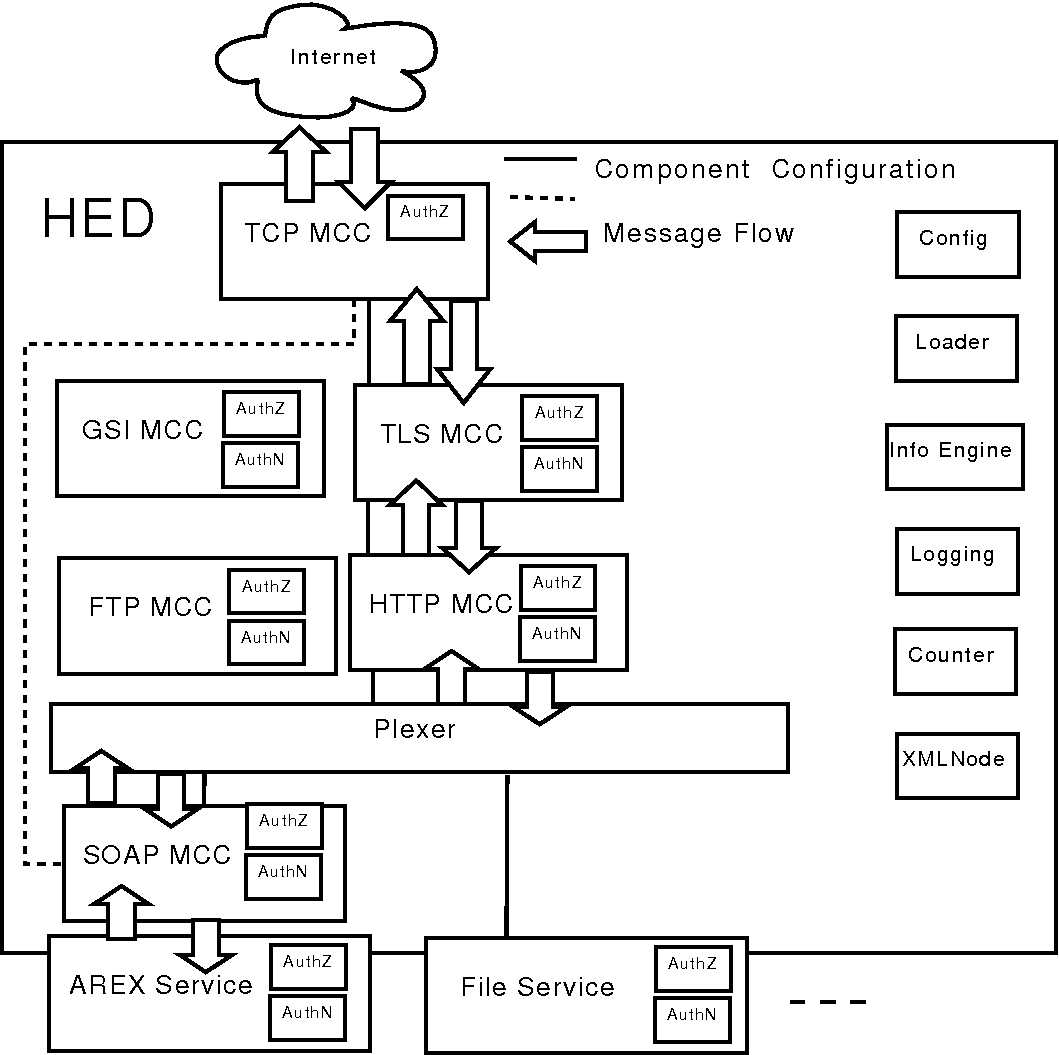
\includegraphics[width=0.75\textwidth]{HED.png}
\caption{The example of Host Environment Daemon deployed with A-REX and File services}
\label{fig:HED}
\end{figure}
HED contains a framework for implementing and enforcing authentication and authorization. Each MCC or Service has a common interface for implementing various authentication and authorization functionality. Each functionality can be implemented as a pluggable and configurable component (plug-ins) called SecHandler, which is implemented as a C++ class and provides a method for processing message that travels through MCC or Service. Each MCC or Service is usually configured with two queues of SecHandler – one for the incoming message and one for the outgoing message respectively. All SecHandler components attached to the queue are executed sequentially. If any of them fails, message processing fails as well. In Figure \ref{fig:HED}, the “AuthZ” and “AuthN” sub-modules inside MCCs and Services are examples of SecHandler.

As explained above, HED is supposed to act as a Web/Grid Service container, but on the client side, from implementation perspective, there is a similar architecture implemented for processing messages from different protocols and handling security functionality; also there is a specific application programming interface (API) for developers to easily write Web Service client code.


\section{Cross-Middleware Authentication and Single Sign-On}
\label{sec:siglesignon}
We investigated the authentication and single sign-on issue in the scenario when a user or user’s representative (acting on behalf of this user) needs to access resources across different middlewares. Our work focuses on the following five major aspects:
Integration of community authentication – to utilize the standard-compatible community authentication mechanism from the Shibboleth~\cite{Shiblink} Identity Provider software when users authenticate against the Grid services.
Short lived credentials service – to issue the short lived X.509 certificates for users authenticated using the community authentication, in order to interoperate with the services that depend on PKI based authentication.
Credential delegation service – to process the X.509 credential delegation as a normal Web Service, in order to provide single sign-on ability.
Message level authentication – to provide message level authentication by implementing WS-Security.
SAML token based delegation service – to process the delegation of an WS Security SAML token in order to provide single sign-on for SOAP message level authentication.


\subsection{Community based authentication for Grid by utilizing Shibboleth Identity Provider}
\label{sec:communityauthn}
AAI (Authentication and Authorization Infrastructure) is a solution for the authentication and authorization in cross-domain resource sharing, such as electronic resource sharing between digital libraries, etc. AAI implicitly applies to the community or institutional based authentication where users from the various communities need to get resources from other communities by using some federation mechanism. Unlike the X.509 based authentication solution in some Grid systems, the AAI does not require users to provide the X.509 certificate, instead, it supports different types of authentication, such as username/password authentication, IP address authentication, etc. There are several implementations of the AAI, among which Shibboleth is the one which has been widely deployed.

The Shibboleth provides cross-domain single sign-on and attribute-based authorization while preserving user privacy. It is based on the OASIS Security Assertion Markup Language (SAML), specifically, the new version of Shibboleth supports SAML 2.0 specification. For the authentication, the Shibboleth implements SAML2.0 web browser SSO profile, which  defines two functional components, an Identity Provider and a Service Provider. The Identity Provider (IdP) is responsible for creating, maintaining, and managing user identity, while the Service Provider (SP) is responsible for controlling access to services and resources by analyzing the SAML assertions produced and issued by the IdP upon request. In order to discover which home community does a user come from, Shibboleth specifies an optional third component called “Where Are You From?” (WAYF) service to aid in the process of IdP discovery. This IdP discovery process is also standardized and defined in SAML 2.0 specification as “Identity Provider Discovery Profile”.

We also utilized the SAML2.0 web browser SSO profile for the authentication in ARC middleware. On the client side the user agent functionality of the Web browser was implemented in order to mimic its behavior, such as the HTTP redirection and the Cookie processing. In fact, implementation of the user agent is also based on the client interface of ARC, specifically, the HTTPS client interface, since the client interface of ARC can support different protocols which are incarnated by different MCCs. On the service side, we implemented the Service Provider functionality (based on the HTTP MCC chained to TLS MCC). For Identity Provider, the Shibboleth IdP implementation is used. Figure \ref{fig:SAML2SSO} shows the process of SAML2.0 SSO integrated in ARC client and service.

\begin{figure}
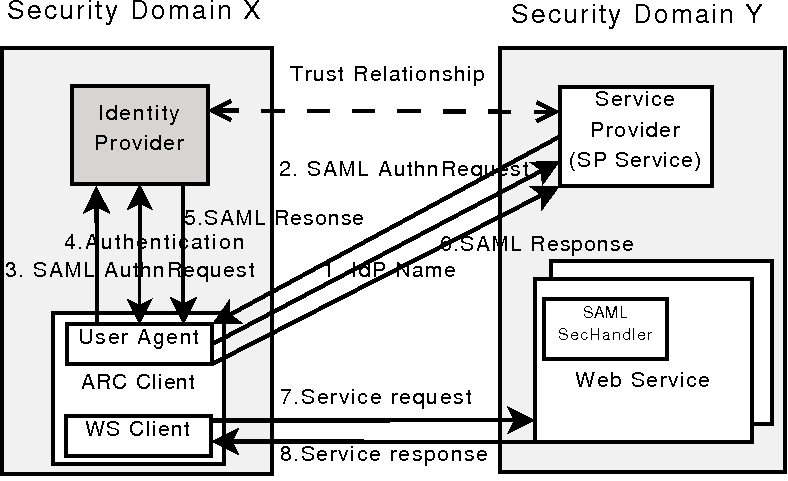
\includegraphics[width=0.75\textwidth]{SAML2SSO.png}
\caption{SAML2.0 SSO profile in ARC}
\label{fig:SAML2SSO}
\end{figure}
Here is the explanation of steps shown in Figure \ref{fig:SAML2SSO}:
1.The client uses the user agent interface to launch a HTTP request including the IdP name (to which the user belongs) to the service side. The endpoint of the SP (Service Provider) service is the same as that of the other target services, except the last part of the endpoint is “saml2sp” which is specific for pointing to the SP Service. Note that we use Identity Provider (IdP) name here to simplify the IdP discovery process in order to avoid the IdP discovery process, because we suppose that the user who would access the target services should better know where is he from initially.
2.The SP Service searches the metadata (we use the same metadata format as defined in the Shibboleth) and gets the location of the single sign-on service (hosted in IdP) and also the location of assertion consuming service (hosted in this SP itself). Then SP Service uses obtained information to compose and issue the SAML authentication request also by utilizing own X.509 certificate (note that in the SAML2.0 SSO profile, X.509 certificates are still needed for IdP and SP) and sends the response back to the user agent.
3.User agent sends the SAML authentication request to the Identity Provider.
4.Identity Provider requires an act of authentication. The authentication mechanism is outside of the SAML2.0 SSO profile. The Shibboleth IdP implementation uses login handlers for authentication. The current user agent implementation is compatible with the Username/Password login handler of Shibboleth IdP. Through the HTTP protocol, the user agent will feed IdP with the username/password which has been given by the caller of user agent interface.
5.Once the authentication has been succeeded, the IdP issues a SAML response including SAML assertion encrypted by destination SP’s public key, and then this SAML response will be delivered by the user agent to the Service Provider.
6.The SP Service verifies and checks the SAML response, decrypts and stores the SAML assertion into session/connection context. That assertion includes the AuthnStatement and AttributeStatement elements.
7.The WS client launches the Grid/Web Service request via the same connection as the one which is used by user agent to contact SP Service.
8.The Grid/Web Service checks the AuthnStatement stored in the session context to see if the session is still valid. If valid, service handles the  request and returns the response to the WS client. Note that in the current implementation the service requires WS client to reuse same TCP connection as the one used by user agent is step 5, in order to guarantee  validity of the SSO result.

The SP service and other functional service(s) are hosted by the same container, and they use the same X.509 credential for the transport layer security. The client authentication may be switched off, so that client doesn’t need to use any X.509 credential. Only the trusted CAs of SP and IdP services need to be configured on the client side to ensure SP and IdP can authentication.

The benefit of the SAML2.0 SSO profile worth mentioning is that the Identity Provider can cache the authentication result through session management once the user agent has succeeded to authenticate. Then for a short period this authentication result is valid so that the user agent doesn’t need to feed IdP with user’s username and password the next time it authenticates against IdP. So the user (or the client on behalf of that user) can travel across multiple security domains with only providing his name and password once, which is the characteristic of single sign-on.

Since the Shibboleth implementation of SAML is standard-compliant and widely deployed, the solution implemented in ARC can interoperate with other SAML implementations with minimum change, and more importantly, this solution can utilize the widely deployed SAML based authentication implementation in Grid systems avoiding the use of X.509 certificate on the client side.


\subsection{Short-Lived Credential Service}
\label{sec:slcs}
However, many widely used Grid middlewares are based on GSI while GSI requires mutual X.509 authentication. Also for Web Service based Grid solutions, we cannot prevent service side from requiring client's X.509 certificate.  Based on the solution described in previous section, we implemented a Short Lived Credential Service (SLCS) through which user can get a short-lived X.509 certificate without being bothered to contact any registration authority (RA) or certificate authority (CA).

\begin{figure}
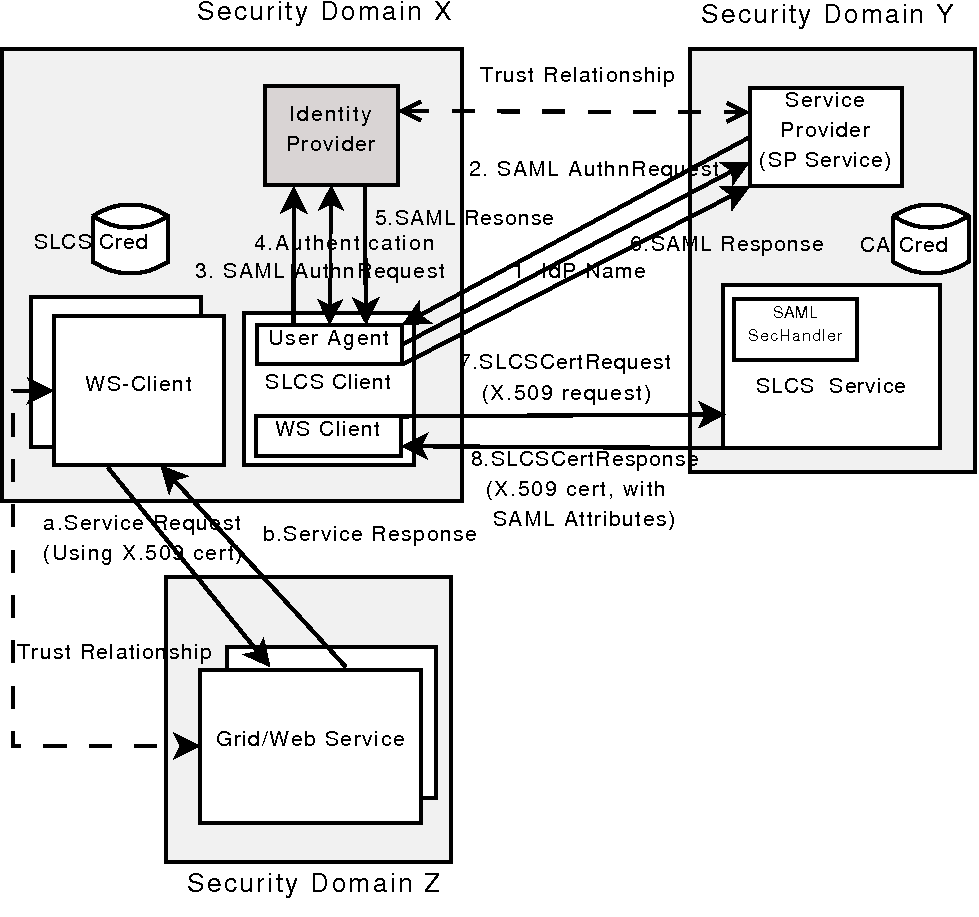
\includegraphics[width=0.75\textwidth]{SLCS.png}
\caption{Short lived credential service}
\label{fig:SLCS}
\end{figure}
The SLCS service is also a Web Service implemented using ARC service interface. The SLCS client is implemented as command-line interface (CLI) utility which implements the user agent and WS client functionalities. The whole process of SLCS invocation is shown in Figure \ref{fig:SLCS} (steps 1‑8). The process resembles one shown in in Figure \ref{fig:SAML2SSO}, except that steps 7 and 8 use SLCS certificate request and response.

The SLCS client sends request to the SLCS service with the generated X.509 certificate request embedded. Upon reception of the request the SLCS service  composes a distinguished name (DN), andissues a certificate (short lived, 12 hours by default) with the SAML attribute (from the SAML2.0 SSO profile) as the X.509 certificate extension and puts the certificate in to the Web Service response. The SLCS client gets the response and stores the X.509 certificate into local repository along with corresponding private key.

Since the lifetime of the short lived credential is usually short, it is not a must to protect the private key by a pass phrase. It is considered enough to use protection  provided by underlying file system. If the private key is not protected by passphrase then it can be used direcctly for steps (a) and (b) in Figure \ref{fig:SLCS} to access Grid Service or Web Service. If the private key is protected, the user can generate temporary  X.509 proxy by using a command-line interface utility such as grid-proxy-init, voms-proxy-init, etc. Then this proxy can by used  to access the Grid/Web Service.

It should be noticed that the process of composing the distinguished name (DN) for the certificate is a critical issue for the SLCS service. Since the Shibboleth Identity Provider uses the eduPerson schema~\cite{eduSchemalink} for the composing the SAML Attribute we pick the relatively distinguishable attribute “eduPersonPrincipalName” for the DN. A typical example of the eduPersonPrincipalName  could be alice@example.org. In such case composed DN is for example “/O=knowarc/OU=example.org/CN=alice”.

The obvious benefit of the SLCS service is that the user can get the X.509 credentials anywhere simply by running the SLCS client command and providing her username and password, and then access the X.509 based Grid infrastructure conveniently. Thanks to the single sign-on capability of SAML2.0 SSO profile, the user doesn’t not need to provide her username and password during valid period after the first time she succeeds to authenticate against her home IdP.


\subsection{X.509 Credential Delegation Service}
\label{sec:creddeleg}
The delegation of credentials proposed in the Grid Security Infrastructure (GSI) is a good solution for supporting single sign-on for users, except that the coupling of the GSI communication is not so widely accepted in Web Service applications. In the design of the new ARC middleware components, we keep the credential delegation idea, while utilizing the SOAP communication (together with TCP or TLS for transport level communication) instead of the GSI communication for the credential delegation process.

As shown in Figure \ref{fig:Delegation}, there is a specific WS client and Web Service for processing delegation: delegation client, and delegation service. The WSDL (Web Service Description Language) of the delegation service has two main operations, one for processing the delegation initiation, and the other for storing the signed proxy certificate. The delegation protocol is detailed in Figure \ref{fig:Delegation_protocol}.

\begin{figure}
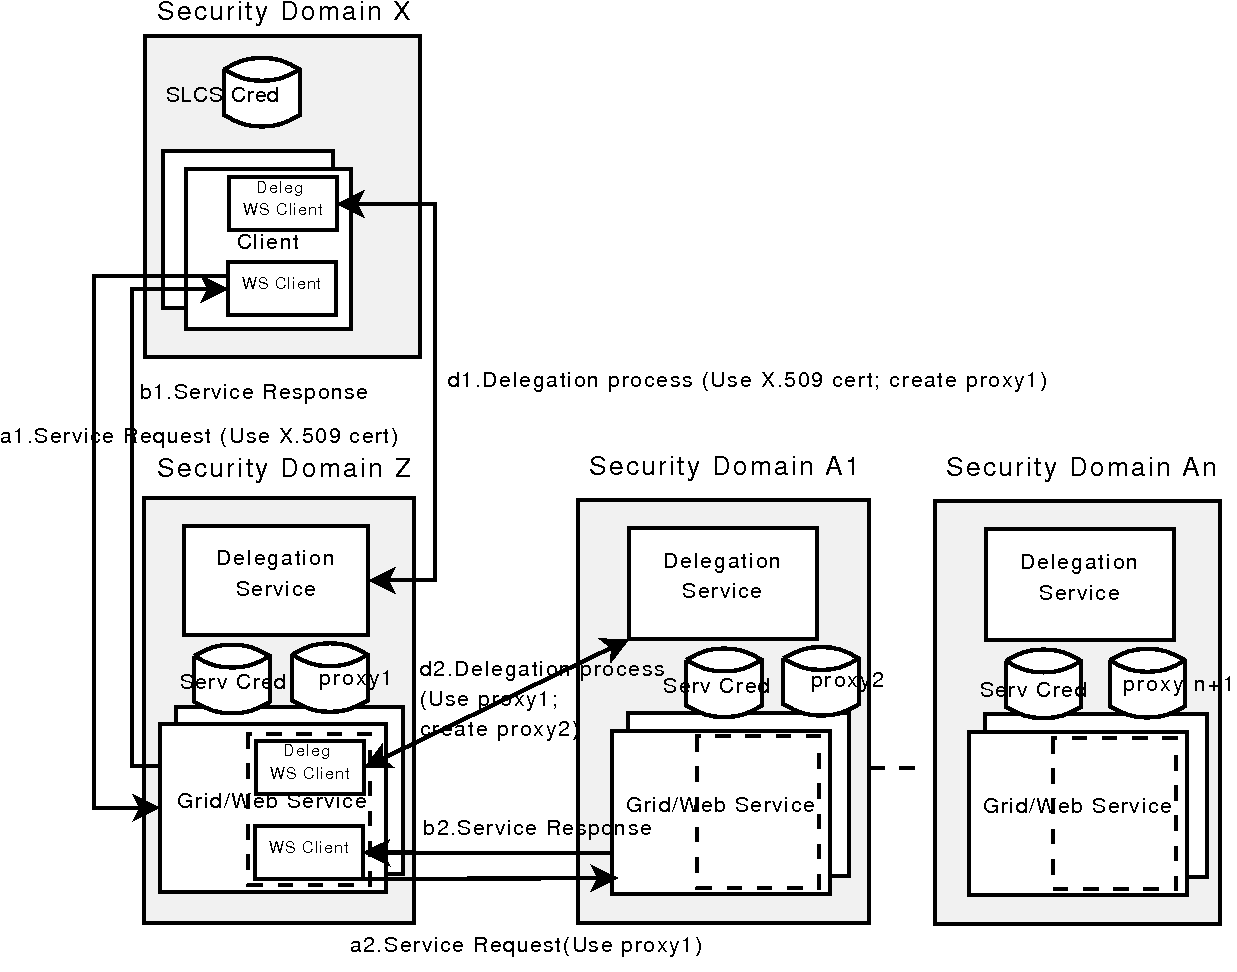
\includegraphics[width=0.75\textwidth]{Delegation.png}
\caption{Credential delegation service and client}
\label{fig:Delegation}
\end{figure}

\begin{figure}
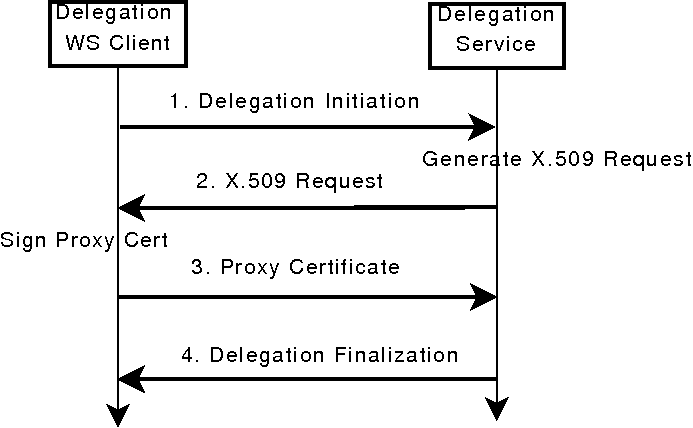
\includegraphics[width=0.75\textwidth]{Delegation_protocol.png}
\caption{Credential delegation protocol}
\label{fig:Delegation_protocol}
\end{figure}
For the delegation process, the delegation WS client functionality (inside each delegation service or the initial client) which is included to access the target delegation service (d1 or d2 in Figure \ref{fig:Delegation}), should use the user’s X.509 credential or a delegated credential (on behalf of the user) for authentication and secure communication, as well as delegate one more level of the delegated credential. For the other general  service invocation process, the WS client functionality (inside each service or the initial client) which is included to access the target service (step a1 or a2 in Figure \ref{fig:Delegation}), should also use the user’s X.509 credential or a delegated credential for authentication and secure communication.

Since each WS client accesses the target service (delegation service or other general services) on behalf of the user, the trust relationship between the user’s certificates (X.509 certificate and proxy certificate) and services is required, while the trust relationship between service’s certificate and another service’s certificate is not required.

What should be mentioned is that the delegation service is also a normal Web Service. Therefore, delegation service implemented in ARC can be accessed by any standard-compliant WS client that intends to delegate credential; also delegation client implemented in ARC can access any other standard-compliant Web Service which accepts delegation request.


\subsection{Message Level Authentication}
\label{sec:msgauthn}
Transport level security (TLS or SSL) is not sufficient for securing Web Service, because the secure channel created by SSL/TLS makes it impossible to differentially protect the SOAP message, e.g. to encrypt or sign only particular components of the SOAP message, which is relevant when non-sensitive portions of the message need to be accessed or changed by intermediate actors. Additionally, SSL/TLS is incapable of providing end-to-end protection for SOAP message which might flow through multiple intermediate actors, because it only allows each hop to be protected with the resultant security gaps at intermediate actors. Web Services Security (WS-Security)~\cite{WSSeclink} specification provides means for applying security to Web Service.

WS-Security related specifications are implemented as SecHandler in ARC. There are three kinds of WS-Security version 1.1 specifications which are completely or partly implemented: Username Token profile, X.509 Token profile, and SAML Token profile.

For those WS clients on behalf of a user, at any step of service invocation, the WS client can augment the SOAP message with WS-Security token by simply configuring the WS-Security SecHandler into container’s configuration, if the relying party (target service) requires.

If the WS client owns an X.509 certificate or proxy certificate, the process of generating an X.509 Token for a SOAP message is: this client puts the content of certificate into X.509 token as <wsse:BinarySecurityToken>, and uses the private key (corresponding to the certificate) to create XML signature for the SOAP message body.

However the process of generating a SAML Token is more complicated. In the WS-Security SAML Token profile, ConfirmationMethod is the verifying method for establishing proof-of-possession for the subject. Two methods are proposed in the SAML Token profile: holder-of-key and sender-vouches. We rely on the holder-of-key method. For the holder-of-key subject confirmation method, there are three interaction parts: the attesting entity, the relying party and the issuing authority. Firstly, the attesting entity authenticates to issuing authority by using some authentication scheme such as X.509 Token profile, or SSL/TLS mutual authentication. Then the issuing authority is able to make a definitive statement (sign a SAML assertion) about an act of authentication that has already taken place. The attesting entity gets the SAML assertion and then signs the SOAP message together with the assertion by using its private key (the relevant certificate has been authenticated by issuing authority, and its relevant public key has been put into the SubjectConfirmation element under SAML assertion by issuing authority). Only the exact entity that possesses the private key which is paired with the public key in the SAML assertion can sign the SOAP message, which establishes an irrefutable connection between the author of the SOAP message and the assertion describing an authentication event.

The relying party is supposed to trust the issuing authority. When it receives a message from the asserting entity, it will check the SAML assertion based on its predetermined trust relationship with the SAML issuing authority, and check the signature of the SOAP message based on the public key in the SAML assertion without directly trust relationship with attesting entity (holder of this public key).
In terms of verification, since the proxy certificates have been introduced in IETF (RFC 3820)~\cite{RFC3820link}, and OpenSSL has also implemented RFC3820, it is not difficult to use the proxy certificate for the X.509 Token profile to issue an X.509 token.


\subsection{SAML Token Delegation Service}
\label{sec:samldeleg}
There is also a delegation requirement on the message level: some entities often need to temporarily delegate themselves to another entity in order to perform actions on their behalf. We propose a delegation mechanism for the SAML Token. Figure \ref{fig:SAMLDelegation} shows the parties of the SAML Token delegation.

\begin{figure}
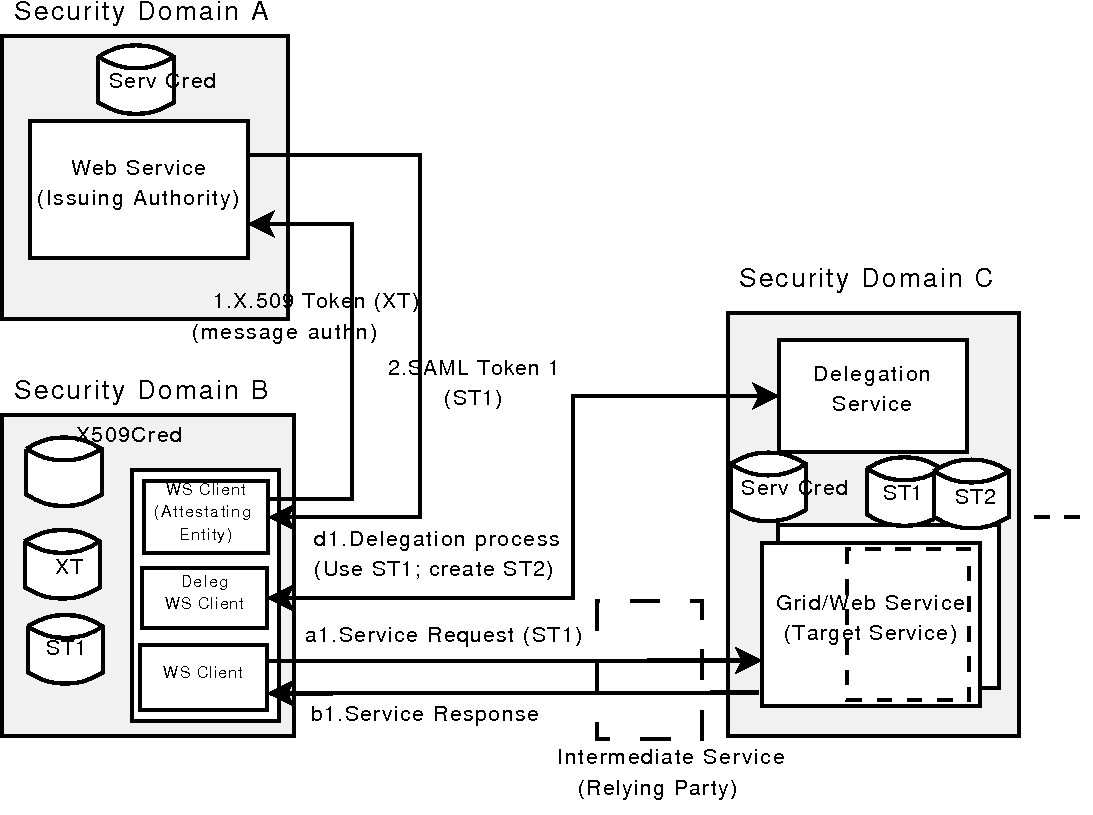
\includegraphics[width=0.75\textwidth]{SAMLDelegation.png}
\caption{SAML Token delegation service and client}
\label{fig:SAMLDelegation}
\end{figure}

\begin{figure}
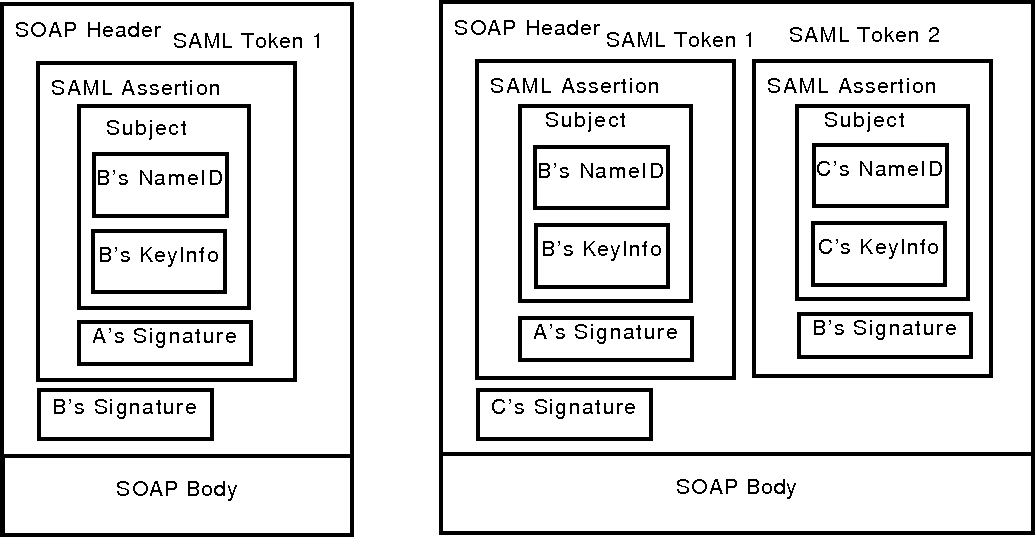
\includegraphics[width=0.75\textwidth]{SAMLDelegationMessage.png}
\caption{SOAP message header with SAML delegation token inside}
\label{fig:SAMLDelegationMessage}
\end{figure}
The delegation process is similar to the process in the X.509 credential delegation service, with the following differences:
1.Transport level communication between delegation client and service is not based on mutual authentication between the proxy certificate and the service certificate; instead, it is based on mutual authentication between the service certificates.
2.Delegation service will not generate any certificate request; instead, the delegation client will pick the public key from the peer certificate after a successful SSL/TLS authentication. So step 2 of the delegation protocol is just some confirmation information which informs delegation client to proceed.
3.For those multiple intermediate services through which a SOAP message flows, delegation service does not need to appear, instead, it only needs to appear on the end of the SOAP message flow.
4.SAML Token might include one or a few <saml:Attribute> attributes which carry the attribute information related to the subject, instead of the Attribute Certificate which is used in the VOMS proxy certificate for carrying the attribute information.

Figure \ref{fig:SAMLDelegationMessage} shows the SAML Token (SAML Assertion) inside the SOAP message is changed due to delegation (we suppose X.509 token is used for attesting entity to authenticate against issuing authority). The SOAP message on the left side is the one which B sends to the relying party (intermediate service). B is the identity of the attesting entity’s X.509 token, while A is the identity of issuing authority, and the SOAP message is signed by B’s private key which is corresponding to the X.509 certificate that is used to create the X.509 token. On the right side, C is the identity of the delegation service (also C is the identity of the target service to which B will access), and now the SOAP message is signed by C’s private key which is corresponding to the target service’s certificate.

What is worth mentioning is: since the SLCS X.509 credential or the delegated credential can be used to issue an X.509 token,  the X.509 credential delegation and SAML Token delegation are smoothly bridged, which benefits the single sign-on.



\section{Related Work}
\label{sec:relatedwork}
Similar work that integrates Shibboleth and Grid middleware does exist. GridShib~\cite{VWelch05},\cite{TBarton06} uses Shibboleth to get entity’s attribute for the authorization of services developed in Globus Tookit. Unlike the work described in this paper, the GridShib does not use Shibboleth’s native login handlers for authentication to Shibboleth IdP, instead, a new login handler specific for X.509 based authentication is developed for the Shibboleth IdP, and a credential service is developed for acting as an online-CA, authenticating the user, and issuing short-lived X.509 credential. Moreover, this paper provides a single sign-on solution for the user with community credentials authenticating to Grid services by directly using SAML2.0 SSO profile.

SWITCH (The Swiss Education and Research Network) short-lived credential service (SLCS)~\cite{switchslcslink} provides a SLCS service and a client. The advantage of our work comparing to the SWTCH’s solution is that the SLCS service and client are based on Web Services, so that they can be implemented in any Web Service container while keeping interoperability.

In terms of delegation, apart from the credential delegation mechanism of GSI~\cite{IFoster98},{VWelch04}, several authors~\cite{MAhsant04} propose a delegation protocol based on the WS-Trust~\cite{WSTrustlink} in order to provide a standard and interoperable protocol for the delegation in Grids. WS-Trust will also be adopted by the ARC middleware to express the specifications required to define delegation protocol in a standard way. Gridsite project implements a X.509 credential delegation solution~\cite{GridSitelink} based on the Web Service, with which ARC delegation client can be made easily interoperable.

GSI plug-in for gSOAP~\cite{GAloisio05} adds GSI support for gSOAP Web Service toolkit. The GSI MCC implemented in ARC provides samilar functionality. Moreover, the ARC solution is more flexible because GSI MCC of both service and client sides is pluggable, which means service and client developers of the ARC do not need to modify the service or client implementation in order to add or replace the GSI functionality.



\section{Conclusion And Future Work}
\label{sec:conclusion}
In this paper we presented the solution built into the ARC Grid middleware, aiming towards the cross-middleware authentication and single sign-on. The goal of our work is to develop an interoperable and accessible single sign-on solution to be used for a VO scenario in production Grids, where users can easily authenticate against the Grids with any of their credentials (not only X.509) from anywhere, and move inside Grid middleware infrastructure and even across heterogeneous Grids  boundaries, without re-authentication within a reasonable period. In order to do so, we implemented some standards based Web Services (including the SLCS service, the X.509 credential delegation service, and the SAML Token delegation service), as well as the user agent and the Service Provider in the context of the SAML2 SSO profile.

It must be noted that due to the standard specifications utilized (SAML and WS-Security) which are independent from any particular middleware, the WS clients and Web/Grid Services developed within the ARC middleware can interoperate with WS clients and Web/Grid Services developed as part of some other middlewares in a standardized way. ARC also supports interoperability with Grid middlewares that require GSI based communication.

Though only authentication issue is discussed in this paper, as the future work, we will implement a solution for cross-middleware attribute-based authorization by using the standard specifications such as SAML.


% Text with citations \cite{RefB} and \cite{RefJ}.
%\subsection{Subsection title}
%\label{sec:2}
%as required. Don't forget to give each section
%and subsection a unique label (see Sect.~\ref{sec:1}).
%\paragraph{Paragraph headings} Use paragraph headings as needed.


%% For one-column wide figures use
%\begin{figure}
%% Use the relevant command to insert your figure file.
%% For example, with the graphicx package use
%  \includegraphics{example.eps}
%% figure caption is below the figure
%\caption{Please write your figure caption here}
%\label{fig:1}       % Give a unique label
%\end{figure}
%%
%% For two-column wide figures use
%\begin{figure*}
%% Use the relevant command to insert your figure file.
%% For example, with the graphicx package use
%  \includegraphics[width=0.75\textwidth]{example.eps}
%% figure caption is below the figure
%\caption{Please write your figure caption here}
%\label{fig:2}       % Give a unique label
%\end{figure*}
%
%% For tables use
%\begin{table}
%% table caption is above the table
%\caption{Please write your table caption here}
%\label{tab:1}       % Give a unique label
%% For LaTeX tables use
%\begin{tabular}{lll}
%\hline\noalign{\smallskip}
%first & second & third  \\
%\noalign{\smallskip}\hline\noalign{\smallskip}
%number & number & number \\
%number & number & number \\
%\noalign{\smallskip}\hline
%\end{tabular}
%\end{table}


\begin{acknowledgements}
We would thank all of the ARC middleware developers for their work. We wish to thank Oxana Smirnova from Lund University for vital comments and proof-reading.
\end{acknowledgements}

% BibTeX users please use one of
%\bibliographystyle{spbasic}      % basic style, author-year citations
%\bibliographystyle{spmpsci}      % mathematics and physical sciences
%\bibliographystyle{spphys}       % APS-like style for physics
%\bibliography{}   % name your BibTeX data base

% Non-BibTeX users please use
\begin{thebibliography}{}
%
% and use \bibitem to create references. Consult the Instructions
% for authors for reference list style.
%
%\bibitem{RefJ}
% Format for Journal Reference
%Author, Article title, Journal, Volume, page numbers (year)
% Format for books
%\bibitem{RefB}
%Author, Book title, page numbers. Publisher, place (year)
% etc

\bibitem{IFoster01}
Foster I, Kesselman C, Tuecke S. The anatomy of the Grid: Enabling scalable virtual organizations, International Journal of Supercomputer Applications, 15(3), 200–222 (2001)

\bibitem{IFoster98}
Foster, I., Kesselman, C., Tsudik, G. and Tuecke, S. A Security Architecture for Computational Grids, ACM Conference on Computers and Security, 1998, 83-91.

\bibitem{AlfieriR05}
R. Alfieri, R. Cecchini, V. Ciaschini, L. dell’Agnello, A. Frohner, K. Lorentey, and F. Spataro. From gridmap-file to voms: managing authorization in a Grid environment. Future Generation Comp. Syst., 21(4), 549–558 (2005)

\bibitem{RFC3821link}
RFC 3821- An Internet Attribute Certificate Profile for Authorization. http://www.faqs.org/rfcs/rfc3281.html

\bibitem{GTlink}
Globus Toolkit. http://www.globus.org/toolkit/

\bibitem{gLitelink}
gLite: lightweight middleware for Grid computing. http://glite.web.cern.ch

\bibitem{ARClink}
Advanced Resource Connector. http://www.nordugrid.org/middleware/

\bibitem{WSSeclink}
OASIS Web Services Security. www.oasis-open.org/committees/wss/

\bibitem{SAMLlink}
OASIS Security Assertion Markup Languages (SAML). www.oasis-open.org/committees/security/

\bibitem{MEllert07}
M. Ellert et al. Advanced resource connector middleware for lightweight computational grids, Future Generation computer systems, 23(2), 219–240 (2007)

\bibitem{KnowARClink}
KnowARC project.  https://www.knowarc.eu/

\bibitem{KnowARCDesignlink}
Design document of new version ARC. https://www.knowarc.eu/documents/Knowarc\_D1.1-1\_07.pdf

\bibitem{WSElink}
Web Services Enhancements 2.0 Service Pack 2. http://msdn.microsoft.com/en-us/library/

\bibitem{AShoshani03}
A. Shoshani, A. Sim, and J. Gu, Storage Resource Managers: Essential Components for the Grid, Grid Resource Management: State of the Art and Future Trends, Kluwer Publishing, 2003.

\bibitem{Shiblink}
The Shibboleth Project. http://shibboleth.internet2.edu/

\bibitem{eduSchemalink}
eduPerson and eduOrg Object shema. http://middleware.internet2.edu/eduperson/

\bibitem{RFC3820link}
Internet X.509 Public Key Infrastructure (PKI) Proxy Certificate Profile. ttp://www.ietf.org/rfc/rfc3820.txt

\bibitem{VWelch05}
V. Welch, T. Barton, K. Keahey and F. Siebenlist. Attributes, Anonymity, and Access: Shibboleth and Globus Integration to Facilitate Grid Collaboration. 4th Annual PKI R\&D Workshop, 2005.

\bibitem{TBarton06}
T. Barton et al. Identity Federation and Attribute-based Authorization through the Globus Toolkit, Shibboleth, Gridshib, and MyProxy. 5th Annual PKI R\&D Workshop, 2006.

\bibitem{switchslcslink}
SWITCH Short Lived Credential Service. http://www.switch.ch/Grid/slcs/

\bibitem{VWelch04}
V. Welch et al. X.509 proxy certificate for dynamic delegation, Proceeding of the 3rd Annual KI R\&D Workshop, 2004.

\bibitem{MAhsant04}
M. Ahsant, J. Basney, and O. Mulmo. Grid Delegation Protocol, UK Workshop on Grid Security Experiences, Oxford. 2004.

\bibitem{WSTrustlink}
OASIS WS-Trust specification. http://docs.oasis-open.org/ws-sx/ws-trust/200512

\bibitem{GridSitelink}
Gridsite delegation service. http://www.gridsite.org/wiki/Delegation\_protocol

\bibitem{GAloisio05}
Giovanni Aloisio, Massimo Cafaro, Italo Epicoco, Daniele Lezzi, and Robert van Engelen, The GSI plug-in for gSOAP: Enhanced Security, Performance, and Reliability, ITCC conference 2005, IEEE Press, Volume I, pages 304-309.

\end{thebibliography}

\end{document}
% end of file template.tex

